\newpage
\subsection{Test 3: File Format Frequency}
A variety of file frequency formats were tested to see how they differed in terms of pause count and pause measurement. 
This test was done using the talkbank file 6269 as it was the best representative of the talkbank files. 
This was done to understand the impact file format frequency had on resulting pause data.  
%As this takes a long time to compute, only a sample of the data was selected for these tests. Of those files there were preliminary tests were done to see what pause data looked like initially from these and the best and worst performers were chosen to see how they change with frequency change. I think 5000, 4894, 4888, something like that were really bad. Essentially the outliers from these graphs. 


%The digitisation of the audiofile required the most amount of time but increased heavily as audio file size increased. \\

\begin{tabular}{ |p{1.8cm}| |p{1.5cm} |p{1.5cm} |p{1.3cm} |p{1.1cm} |p{1.4cm} |p{1.5cm} |p {1.4cm} |}
	\hline
	\multicolumn{8}{|c|}{CallFriend - English (Northern) - 6269} \\%
	\hline
	{\small Audio File} & 
	{\footnotesize Time taken (min:sec)} & 
	{\footnotesize Binary Pause Array Length} & 
	{\footnotesize Total Audio Pause} & 
	{\footnotesize Total Sounding} & 
	{\footnotesize Pause Proportion} & 
	{\footnotesize Num. of Pauses} & 
	{\footnotesize Avg. Pause Length} \\
		\hline\hline
		%\cellcolor[HTML]{A2A1A2} 
%		8000 & 00:00 & xxxxx & xxxxx & xxx & xx.xx\% & xxx  & xx.xx \\
%		\hline 
		11025 & 02:16 & 18040 & 17367 & 673 & 96.27\% & 507  & 3425ms \\
		\hline 
		\rowcolor{lightgray} 
		16000 & 03:40 & 17999 & 17348 & 651 & 96.38\% & 496 & 3498ms \\
		\hline
		22050 & 04:48 & 18040 & 17362 & 678 & 96.24\% & 510 & 3404ms \\
		\hline
		32000 & 07:01 & 17999 & 17336 & 663 & 96.32\% & 503 & 3447ms \\
		\hline
		44100 & 9:30 & 17999 & 17332 & 667 & 96.30\% & 507 & 3419ms \\
		\hline
		48000& 11:27 & 17999 & 17336 & 663 & 96.32\% & 504 & 3440ms \\
		\hline
		88200 & 13:32 & 17999 & 17333 & 666 & 96.30\% & 503 & 3446ms \\
		\hline
		96000 & 15:42 & 17999 & 17334 & 665 & 96.31\% & 505 & 3432ms \\
		\hline
%		Average & --:-- & . & . & . & . \% & . & . \\
%		\hline
\end{tabular}
\caption{Table: Pause results for various file frequency formats for talkbank file 6269} \\
\label{tab:1}


No significant change was noticeable amongst differing file frequencies. 16,000hz was used as the frequency for talkbank files
%this file 6269 was chosen as it was shown to be a good average file in terms of pause value return. 


%
%
%\begin{figure}[htbp]
%	\begin{center}
%		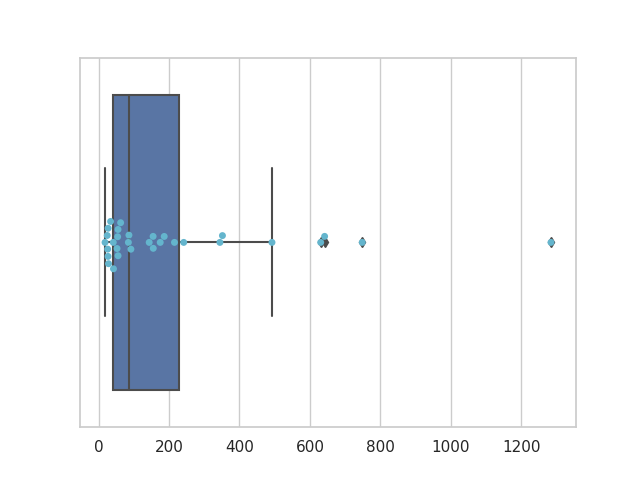
\includegraphics[scale=0.1]{src/main-matter/results/preliminary-testing/frequency/avg_pause_length_all}
%		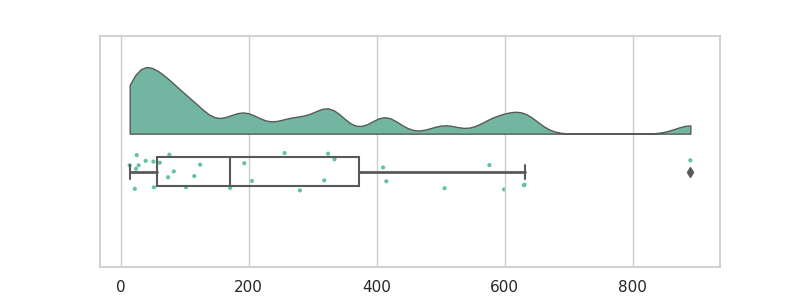
\includegraphics[scale=0.1]{src/main-matter/results/preliminary-testing/frequency/raincloud-pause-groups-num-all}
%		\caption{Where are the labels lmao?}
%		\label{default}
%	\end{center}
%\end{figure}